\section{Wall-resolved turbulence-model results}
\label{sec:comparative:zpg:wall-resolved-baselines}

The first comparison establishes the accuracy of the flow calculation before a wall function is introduced. Wall-resolved Spalart--Allmaras (SA) and \(k\)--\(\omega\) SST simulations are evaluated against the selected DNS references using the matching procedure and transport properties in Section~\ref{sec:evaluation:benchmark-cases}. Both momentum closures use the same gradient-diffusion thermal closure with \(Pr_t=0.9\), unless explicitly stated otherwise. The SA calculations employ the corrected compressible implementation described in Section~\ref{subsec:ext:spalart-allmaras-of-correction}. SA is also the underlying momentum closure for the coupled Li and Griffin calculations investigated subsequently, whereas SST provides a general comparison with another widely used RANS model.
\par\medskip

The mesh studies in Section~\ref{sec:evaluation:mesh-families-yplus}, provide the basis for using these solutions as wall-resolved references. Their differences from DNS measure the accuracy of the complete resolved RANS calculation, including its thermal closure and remaining numerical and reference-data uncertainties. In the later wall-function comparisons, the corresponding SA solution serves as the baseline against which the additional effects of the wall closure and its coupling to the discretized flow are assessed.

\subsection{Prediction of wall heat-flux and skin-friction}
\label{subsec:comparative:zpg:wr-wall-fluxes}

Table~\ref{tab:wall-resolved:coefficients} reports the, wall coefficients and signed relative errors for both models, across the investigated ZPG FPs at the respectively \(Re_{\delta2}\) matched station. DNS rows give the reference values used to calculate the errors, complementing the published-data overview in Table~\ref{tab:evaluation:dns-reference-values}. The CFD stations agree with the nominal DNS targets to within \(0.1\%\). Overall Table~\ref{tab:wall-resolved:coefficients} shows a relative errors against DNS range from \(-14.8\%\) to \(+13.7\%\) in heat-flux and from \(-18.5\%\) to \(+12.5\%\) in wall shear stress for SA, compared with \(-12.8\%\) to \(+20.6\%\) and \(-17.1\%\) to \(+15.6\%\), respectively, for \(k\)--\(\omega\) SST, across the investigated cases. Neither turbulence model consistently outperforms the other across the investigated cases and wall quantities.

% Table provenance (WSL; absolute paths):
%   /home/mgnadlinger/Duan_DNS_ZPGFP/dns_comparison_{SA,kwSST}/scalar_error_summary.csv
%   /home/mgnadlinger/Zhang_DNS_ZPGFP/dns_comparison_{SA,kwSST}/scalar_error_summary.csv
%   /home/mgnadlinger/Huang_DNS_ZPGFP/dns_comparison_{SA,kwSST}/scalar_error_summary.csv
%   Actual stations checked against the curated results.json files and the combined
%   SA/kwSST profile exports used by the main text and Appendix_ZPG.
%   M5T1 uses the corrected Tw=228.1 K run, also used by its appendix profile.
%   Reproducible extraction and checks: tmp/wall_resolved_table/ (workspace root).
%   RANS -Bq uses the same native Re_delta2-matched results.json samples:
%     /home/mgnadlinger/Zhang_DNS_ZPGFP/{SA,kwSST}_Prt0p9/<case>/postProcessing/TM_ZPGFP/<time>/results.json
%     /home/mgnadlinger/Huang_DNS_ZPGFP/{SA,kwSST}_Prt0p9/M11Tw20/postProcessing/TM_ZPGFP/<time>/stations/<BL>/results.json
%   -Bq = heat_flux_to_wall/(rho_wall*Cp*u_tau*T_wall), with heat_flux_to_wall
%   equal to minus the OpenFOAM wallHeatFlux output. Each RANS wall state is used.
%   Exact paths, times, wall inputs and source hashes: tmp/wall_resolved_table/bq_results_audit.json.
%   Reproduction: tmp/wall_resolved_table/extract_bq.py (workspace root).
% End table provenance.
\begingroup
\small
\sisetup{detect-weight=true}
\setlength{\tabcolsep}{5pt}
\begin{longtable}{@{}ll
    S[table-format=4.1]
    S[table-format=1.5]
    S[table-format=+2.2]
    S[table-format=1.5]
    S[table-format=+2.2]
    S[table-format=1.4]@{}}
    \caption[Wall-resolved wall coefficients and signed DNS errors]{Wall-resolved SA and \(k\)--\(\omega\) SST results at \(Pr_t=0.9\), with the DNS values used for comparison (see Table~\ref{tab:evaluation:dns-reference-values}). The \(Re_{\delta2}\) column gives the nominal target for DNS and the actual sampled value for each CFD solution. Errors \(\varepsilon_f\) and \(\varepsilon_h\) are \(100(C_{\mathrm{RANS}}-C_{\mathrm{DNS}})/C_{\mathrm{DNS}}\) for \(C_f\) and \(C_h\), respectively. The \(-B_q\) column gives Zhang~\cite[Table~2]{zhang2018direct} and Huang~\cite[Table~3]{huang2020simulation} DNS values and corresponding RANS values \(q_{\mathrm{to\,wall}}/(\rho_w c_p u_\tau T_w)\), using heat-flux positive into the wall and each solution's wall state. Entries for \(C_h\) and \(\varepsilon_h\) are omitted for the adiabatic references M5T5 and M2p5 and for M6Tw076; these omissions do not imply zero RANS heat-flux.}\label{tab:wall-resolved:coefficients}\\
    \toprule
    Case / station & Model & {\(Re_{\delta2}\)} & {\(10^3 C_f\)} & {\(\varepsilon_f\,[\%]\)} & {\(10^3 C_h\)} & {\(\varepsilon_h\,[\%]\)} & {\(-B_q\)} \\
    \midrule
    \endfirsthead
    \multicolumn{8}{@{}l}{\tablename~\thetable\ (continued)}\\
    \toprule
    Case / station & Model & {\(Re_{\delta2}\)} & {\(10^3 C_f\)} & {\(\varepsilon_f\,[\%]\)} & {\(10^3 C_h\)} & {\(\varepsilon_h\,[\%]\)} & {\(-B_q\)} \\
    \midrule
    \endhead
    \midrule
    \multicolumn{8}{r@{}}{Continued on next page}\\
    \endfoot
    \bottomrule
    \endlastfoot
    \multicolumn{8}{@{}l}{\textit{Martin--Duan Part 2}}\\*
    \multirow{3}{*}{M5T1} & \textbf{DNS} & \bfseries 1538.4 & \bfseries 2.46 & {\textbf{\textemdash}} & \bfseries 1.39 & {\textbf{\textemdash}} &  \\*
     & SA & 1538.5 & 2.0055 & -18.48 & 1.1839 & -14.83 &  \\*
     & SST & 1538.4 & 2.2824 & -7.22 & 1.3429 & -3.39 &  \\
    \addlinespace[3pt]
    \multirow{3}{*}{M5T2} & \textbf{DNS} & \bfseries 1521.5 & \bfseries 2.05 & {\textbf{\textemdash}} & \bfseries 1.14 & {\textbf{\textemdash}} &  \\*
     & SA & 1520.8 & 1.7334 & -15.45 & 1.0144 & -11.02 &  \\*
     & SST & 1522.2 & 1.7967 & -12.35 & 1.0531 & -7.62 &  \\
    \addlinespace[3pt]
    \multirow{3}{*}{M5T3} & \textbf{DNS} & \bfseries 1524.7 & \bfseries 1.81 & {\textbf{\textemdash}} & \bfseries 0.977 & {\textbf{\textemdash}} &  \\*
     & SA & 1525.0 & 1.5229 & -15.86 & 0.8763 & -10.30 &  \\*
     & SST & 1525.5 & 1.5003 & -17.11 & 0.8697 & -10.98 &  \\
    \addlinespace[3pt]
    \multirow{3}{*}{M5T4} & \textbf{DNS} & \bfseries 1526.4 & \bfseries 1.5 & {\textbf{\textemdash}} & \bfseries 0.839 & {\textbf{\textemdash}} &  \\*
     & SA & 1525.9 & 1.3674 & -8.84 & 0.7545 & -10.07 &  \\*
     & SST & 1526.2 & 1.3018 & -13.22 & 0.7320 & -12.76 &  \\
    \addlinespace[3pt]
    \multirow{3}{*}{M5T5} & \textbf{DNS} & \bfseries 1536.8 & \bfseries 1.28 & {\textbf{\textemdash}} & {\textbf{\textemdash}} & {\textbf{\textemdash}} &  \\*
     & SA & 1537.3 & 1.1912 & -6.94 & {\textemdash} & {\textemdash} &  \\*
     & SST & 1536.8 & 1.1032 & -13.81 & {\textemdash} & {\textemdash} &  \\
    \addlinespace[3pt]
    \multicolumn{8}{@{}l}{\textit{Martin--Duan Part 4}}\\*
    \multirow{3}{*}{LowH\_M3} & \textbf{DNS} & \bfseries 1554.5 & \bfseries 3.12 & {\textbf{\textemdash}} & \bfseries 1.82 & {\textbf{\textemdash}} &  \\*
     & SA & 1554.4 & 2.8950 & -7.21 & 1.7187 & -5.56 &  \\*
     & SST & 1555.0 & 3.5183 & +12.77 & 2.0712 & +13.80 &  \\
    \addlinespace[3pt]
    \multicolumn{8}{@{}l}{\textit{Zhang}}\\*
    \multirow{3}{*}{M2p5} & \textbf{DNS} & \bfseries 1657 & \bfseries 2.3125 & {\textbf{\textemdash}} & {\textbf{\textemdash}} & {\textbf{\textemdash}} & {\textbf{\textemdash}} \\*
     & SA & 1658.0 & 2.1858 & -5.48 & {\textemdash} & {\textemdash} & {\textemdash} \\*
     & SST & 1656.5 & 2.0949 & -9.41 & {\textemdash} & {\textemdash} & {\textemdash} \\
    \addlinespace[3pt]
    \multirow{3}{*}{M6Tw025} & \textbf{DNS} & \bfseries 1135 & \bfseries 1.7043 & {\textbf{\textemdash}} & \bfseries 1.0215 & {\textbf{\textemdash}} & \bfseries 0.14 \\*
     & SA & 1135.3 & 1.6172 & -5.11 & 0.9659 & -5.44 & 0.1320 \\*
     & SST & 1135.8 & 1.7563 & +3.05 & 1.0507 & +2.86 & 0.1374 \\
    \addlinespace[3pt]
    \multirow{3}{*}{M6Tw076} & \textbf{DNS} & \bfseries 1746 & \bfseries 0.99785 & {\textbf{\textemdash}} & {\textbf{\textemdash}} & {\textbf{\textemdash}} & \bfseries 0.02 \\*
     & SA & 1746.2 & 1.0120 & +1.42 & {\textemdash} & {\textemdash} & {\textemdash} \\*
     & SST & 1746.2 & 0.9419 & -5.60 & {\textemdash} & {\textemdash} & {\textemdash} \\
    \addlinespace[3pt]
    \multirow{3}{*}{M8Tw048} & \textbf{DNS} & \bfseries 1990 & \bfseries 0.76629 & {\textbf{\textemdash}} & \bfseries 0.44856 & {\textbf{\textemdash}} & \bfseries 0.06 \\*
     & SA & 1989.9 & 0.8010 & +4.53 & 0.4710 & +5.01 & 0.0592 \\*
     & SST & 1990.0 & 0.7691 & +0.37 & 0.4563 & +1.73 & 0.0586 \\
    \addlinespace[3pt]
    \multirow{3}{*}{M14Tw018} & \textbf{DNS} & \bfseries 2354 & \bfseries 0.40395 & {\textbf{\textemdash}} & \bfseries 0.24337 & {\textbf{\textemdash}} & \bfseries 0.19 \\*
     & SA & 2354.6 & 0.4545 & +12.52 & 0.2694 & +10.70 & 0.1825 \\*
     & SST & 2354.0 & 0.4668 & +15.57 & 0.2776 & +14.09 & 0.1851 \\
    \addlinespace[3pt]
    \multicolumn{8}{@{}l}{\textit{Huang M11Tw020}}\\*
    \multirow{3}{*}{BL1} & \textbf{DNS} & \bfseries 2204 & \bfseries 0.61 & {\textbf{\textemdash}} & \bfseries 0.36 & {\textbf{\textemdash}} & \bfseries 0.164 \\*
     & SA & 2204.5 & 0.6332 & +3.80 & 0.3760 & +4.44 & 0.1647 \\*
     & SST & 2203.2 & 0.6623 & +8.57 & 0.3941 & +9.46 & 0.1683 \\
    \addlinespace[3pt]
    \multirow{3}{*}{BL2} & \textbf{DNS} & \bfseries 3419 & \bfseries 0.55 & {\textbf{\textemdash}} & \bfseries 0.316 & {\textbf{\textemdash}} & \bfseries 0.154 \\*
     & SA & 3418.8 & 0.5820 & +6.40 & 0.3458 & +9.44 & 0.1587 \\*
     & SST & 3418.8 & 0.6140 & +12.24 & 0.3652 & +15.57 & 0.1627 \\
    \addlinespace[3pt]
    \multirow{3}{*}{BL3} & \textbf{DNS} & \bfseries 4390 & \bfseries 0.51 & {\textbf{\textemdash}} & \bfseries 0.29 & {\textbf{\textemdash}} & \bfseries 0.148 \\*
     & SA & 4389.9 & 0.5545 & +8.73 & 0.3296 & +13.66 & 0.1553 \\*
     & SST & 4389.2 & 0.5884 & +15.37 & 0.3499 & +20.64 & 0.1595 \\
    \addlinespace[3pt]
\end{longtable}
\endgroup

Figures~\ref{fig:wall-resolved:kwSST_DNS_ZPG_FPs} and~\ref{fig:wall-resolved:SA_DNS_ZPG_FPs} summarize the signed errors in the skin-friction coefficient \(C_f\) and Stanton number \(C_h\). The two abscissae characterize different aspects of the flow: \(-B_q\) represents wall heat-transfer, while \(M_\tau\) indicates the strength of compressibility associated with the friction velocity. The Figures~\ref{fig:wall-resolved:kwSST_DNS_ZPG_FPs} and~\ref{fig:wall-resolved:SA_DNS_ZPG_FPs} do not reveal any clear correlation in reduction in error with either cold-wall effect or compressibility. Thus from this investigation it is unclear what causes the turbulence models to have such bad performance in predicting the heat-flux and skin-friction on hypersonic flat-plates. These comparisons therefore establish a substantial baseline discrepancy on some of the simplest attached turbulent flows, but do not by themselves identify its physical cause.

\begin{figure}[H]
    \centering
    % Figure provenance (WSL; absolute paths):
    %   Original retained figure: /home/mgnadlinger/ZPG_FP_overview/orig.DNS_Cf_Ch_relative_error_kwSST.png
    %   Updated figure: tmp/wall_resolved_table/figures/DNS_Cf_Ch_relative_error_kwSST.png (workspace root)
    %   Readability replot (2026-10-19): four stacked panels at the printed 170 mm
    %     width, 9.5 pt labels/ticks/legend, and vector PDF output. Exact values and
    %     omissions are retained from the audited 2026-10-14 figures above.
    %     Local regeneration: Figures/WallResolved/plot_wall_coefficient_errors.py
    %     with wall_coefficient_error_data.csv and wall_coefficient_error_provenance.json
    %     in the same directory (paths relative to this chapter).
    %   Python script:
    %     /home/mgnadlinger/ZPG_FP_overview/plot_dns_coefficient_errors.py
    %   Data / simulation roots (high-level):
    %     /home/mgnadlinger/Duan_DNS_ZPGFP/dns_comparison_kwSST
    %     /home/mgnadlinger/Huang_DNS_ZPGFP/dns_comparison_kwSST
    %     /home/mgnadlinger/Zhang_DNS_ZPGFP/dns_comparison_kwSST
    %     /home/mgnadlinger/Duan_DNS_ZPGFP/Martin_Duan_Part2/kwSST_Prt0p9
    %     /home/mgnadlinger/Duan_DNS_ZPGFP/Martin_Duan_Part4/kwSST_Prt0p9/LowH_M3
    %     /home/mgnadlinger/Huang_DNS_ZPGFP/kwSST_Prt0p9/M11Tw20
    %     /home/mgnadlinger/Zhang_DNS_ZPGFP/kwSST_Prt0p9
    %     /home/mgnadlinger/Duan_DNS_ZPGFP/Martin_Duan_Part2/Digitizations
    %     /home/mgnadlinger/Duan_DNS_ZPGFP/Martin_Duan_Part4/Digitizations
    %     /home/mgnadlinger/Huang_DNS_ZPGFP/References
    %     /home/mgnadlinger/Zhang_DNS_ZPGFP/References/Data
    %   Note: Updated on 2026-10-14 from the current curated comparison exports to include
    %     the corrected M5T1 Tw=228.1 K run, consistent with its appendix profile.
    %     Regeneration wrapper: tmp/wall_resolved_table/regenerate_point_only_overviews.py
    %     (workspace root); retains point-only presentation and original legend, without
    %     the trend fits added to the current external plotting script. All other values
    %     agree with the retained orig. export. Numerical audit and input snapshot are
    %     retained in tmp/wall_resolved_table/; original WSL provenance is preserved above.
    % End figure provenance.
    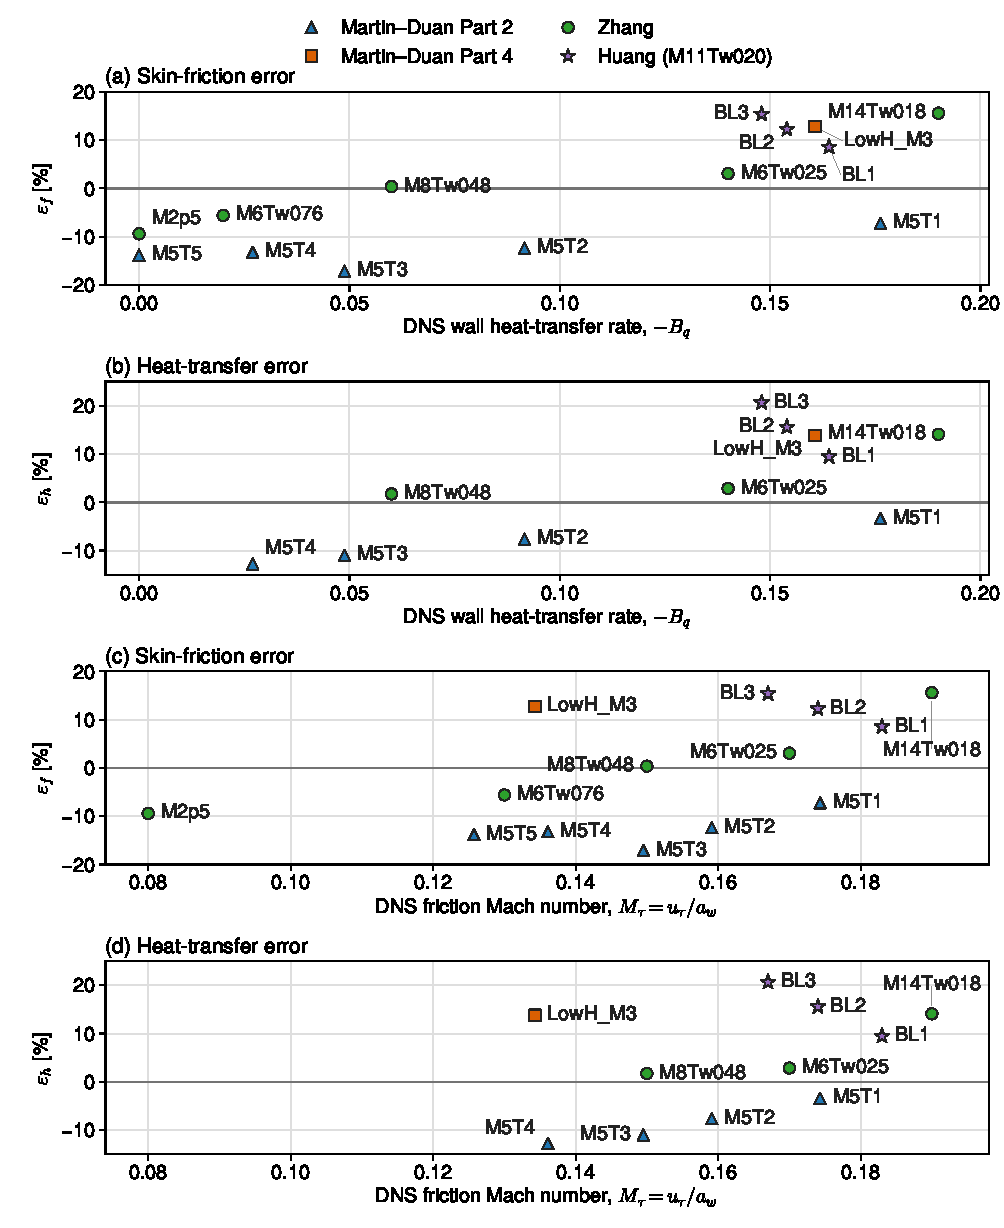
\includegraphics[width=\linewidth]{07_Error_Isolation_Results/Figures/WallResolved/DNS_Cf_Ch_relative_error_kwSST.pdf}
    \caption[Wall-resolved \(k\)--\(\omega\) SST errors in skin-friction and heat-transfer]{Signed relative errors, \(100(C_{\mathrm{RANS}}-C_{\mathrm{DNS}})/C_{\mathrm{DNS}}\), for wall-resolved \(k\)--\(\omega\) SST at \(Pr_t=0.9\). Panels (a,b): errors in the skin-friction coefficient \(C_f\) and Stanton number \(C_h\), respectively, versus the DNS dimensionless wall heat-transfer rate \(-B_q\). Panels (c,d): the corresponding errors versus the DNS friction Mach number \(M_\tau=u_\tau/a_w\). Symbols identify the DNS sources and annotations the cases; BL1--BL3 are three stations of the single Huang case. Heat-transfer errors are omitted for the adiabatic references and M6Tw076. Definitions, matching stations and reference-data limitations follow Section~\ref{sec:evaluation:benchmark-cases}.}
    \label{fig:wall-resolved:kwSST_DNS_ZPG_FPs}
\end{figure}

\begin{figure}[H]
    \centering
    % Figure provenance (WSL; absolute paths):
    %   Original retained figure: /home/mgnadlinger/ZPG_FP_overview/orig.DNS_Cf_Ch_relative_error_SA.png
    %   Updated figure: tmp/wall_resolved_table/figures/DNS_Cf_Ch_relative_error_SA.png (workspace root)
    %   Readability replot (2026-10-19): four stacked panels at the printed 170 mm
    %     width, 9.5 pt labels/ticks/legend, and vector PDF output. Exact values and
    %     omissions are retained from the audited 2026-10-14 figures above.
    %     Local regeneration: Figures/WallResolved/plot_wall_coefficient_errors.py
    %     with wall_coefficient_error_data.csv and wall_coefficient_error_provenance.json
    %     in the same directory (paths relative to this chapter).
    %   Python script:
    %     /home/mgnadlinger/ZPG_FP_overview/plot_dns_coefficient_errors.py
    %   Data / simulation roots (high-level):
    %     /home/mgnadlinger/Duan_DNS_ZPGFP/dns_comparison_SA
    %     /home/mgnadlinger/Huang_DNS_ZPGFP/dns_comparison_SA
    %     /home/mgnadlinger/Zhang_DNS_ZPGFP/dns_comparison_SA
    %     /home/mgnadlinger/Duan_DNS_ZPGFP/Martin_Duan_Part2/SA_Prt0p9
    %     /home/mgnadlinger/Duan_DNS_ZPGFP/Martin_Duan_Part4/SA_Prt0p9/LowH_M3
    %     /home/mgnadlinger/Huang_DNS_ZPGFP/SA_Prt0p9/M11Tw20
    %     /home/mgnadlinger/Zhang_DNS_ZPGFP/SA_Prt0p9
    %     /home/mgnadlinger/Duan_DNS_ZPGFP/Martin_Duan_Part2/Digitizations
    %     /home/mgnadlinger/Duan_DNS_ZPGFP/Martin_Duan_Part4/Digitizations
    %     /home/mgnadlinger/Huang_DNS_ZPGFP/References
    %     /home/mgnadlinger/Zhang_DNS_ZPGFP/References/Data
    %   Note: Updated on 2026-10-14 from the current curated comparison exports to include
    %     the corrected M5T1 Tw=228.1 K run, consistent with its appendix profile.
    %     Regeneration wrapper: tmp/wall_resolved_table/regenerate_point_only_overviews.py
    %     (workspace root); retains point-only presentation and original legend, without
    %     the trend fits added to the current external plotting script. All other values
    %     agree with the retained orig. export. Numerical audit and input snapshot are
    %     retained in tmp/wall_resolved_table/; original WSL provenance is preserved above.
    % End figure provenance.
    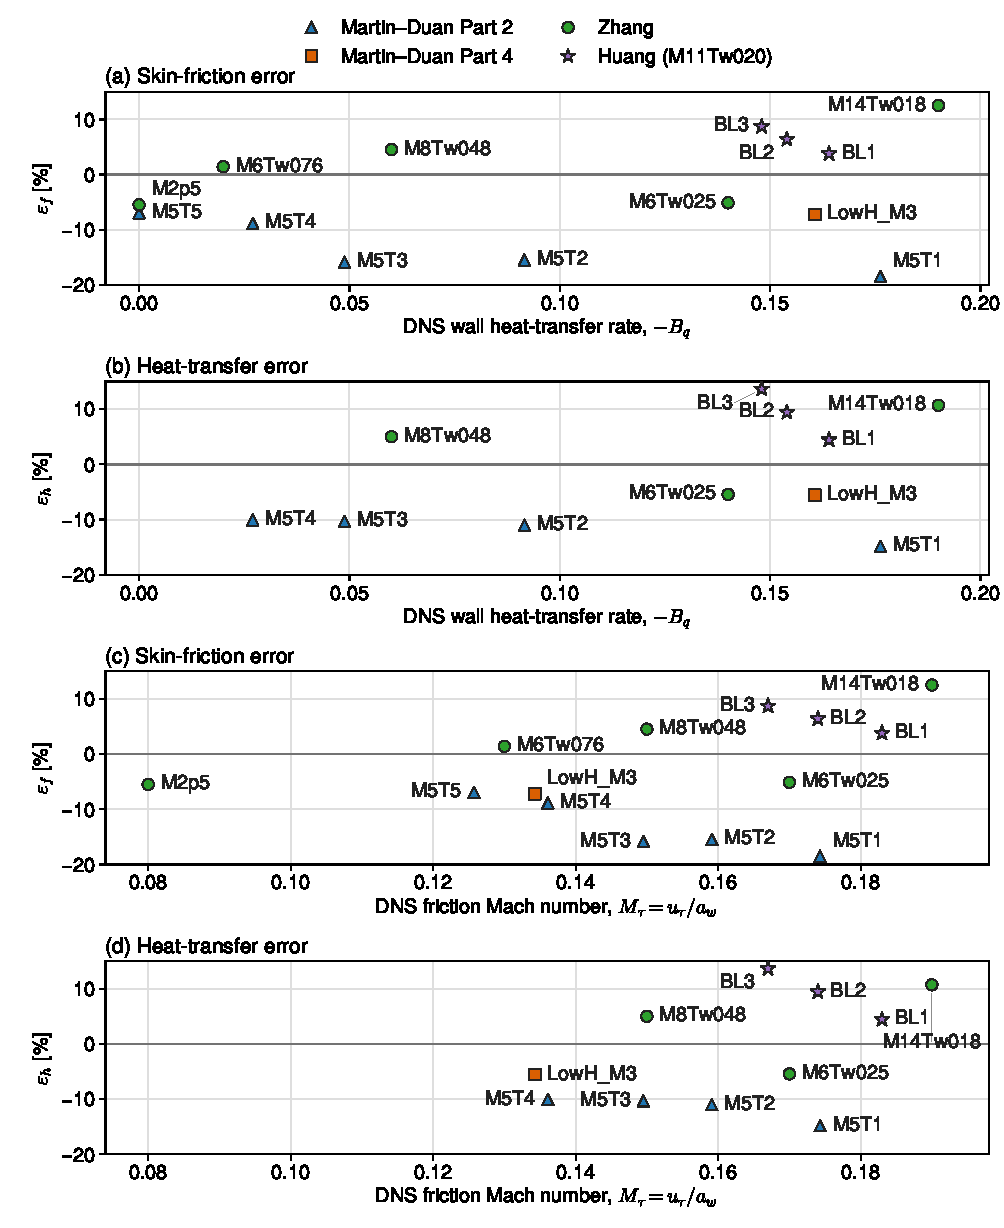
\includegraphics[width=\linewidth]{07_Error_Isolation_Results/Figures/WallResolved/DNS_Cf_Ch_relative_error_SA.pdf}
    \caption[Wall-resolved Spalart--Allmaras errors in skin-friction and heat-transfer]{Signed relative errors for the corrected wall-resolved Spalart--Allmaras model at \(Pr_t=0.9\), using the same references and definitions as Figure~\ref{fig:wall-resolved:kwSST_DNS_ZPG_FPs}. Panels (a,b): errors in \(C_f\) and \(C_h\), respectively, versus DNS \(-B_q\). Panels (c,d): the corresponding errors versus DNS \(M_\tau\). Positive values indicate overprediction of the reference coefficient. Heat-transfer errors are omitted for the adiabatic references and M6Tw076.}
    \label{fig:wall-resolved:SA_DNS_ZPG_FPs}
\end{figure}

\subsection{Boundary layer profiles and temperature--velocity relations}
\label{subsec:comparative:zpg:wr-profiles}

Wall coefficients alone do not show whether the flow supplied to a wall function has the correct internal structure. The detailed profile comparisons therefore examine both velocity and temperature, with particular emphasis on the mean temperature--velocity relation \(T(U)\) introduced in Section~\ref{subsec:background:temperature-velocity}. This relation is directly relevant to the energy closures of the investigated analytical wall functions. A discrepancy in \(T(U)\) implies that a wall closure fitted to DNS and the resolved RANS field need not describe the same relation between thermal and momentum transport, even when their wall heat-fluxes are close.
\par\medskip

Figures~\ref{fig:wall-resolved:M6Tw025_BL_Profile} and~\ref{fig:wall-resolved:LowH_M3_BL_Profile} illustrate the contrast using M6Tw025 and LowH\_M3. Corresponding comparisons for the other ten benchmark cases are provided in Appendix~\ref{app:zpg:wr-profiles}.

\begin{figure}[H]
    \centering
    % Figure provenance (WSL; absolute paths):
    %   Figure: /home/mgnadlinger/Zhang_DNS_ZPGFP/dns_comparison_SA_kwSST/figures/M6Tw025_profiles.png
    %   Python script:
    %     /home/mgnadlinger/Zhang_DNS_ZPGFP/plot_combined_dns_profiles.py
    %   Data / simulation roots (high-level):
    %     /home/mgnadlinger/Zhang_DNS_ZPGFP/SA_Prt0p9/M6Tw025
    %     /home/mgnadlinger/Zhang_DNS_ZPGFP/kwSST_Prt0p9/M6Tw025
    %     /home/mgnadlinger/Zhang_DNS_ZPGFP/References/Data
    %   Print-size replot (2026-10-19):
    %     thesis/07_Error_Isolation_Results/Figures/WallResolved/plot_wall_resolved_profiles.py
    %     Exact plotted coordinates and source hashes retained in adjacent
    %     wall_resolved_profile_data.json and wall_resolved_profile_provenance.json.
    %     Original curves/stations/panel selection preserved; 170 mm PDF, 10.5 pt text.
    % End figure provenance.
    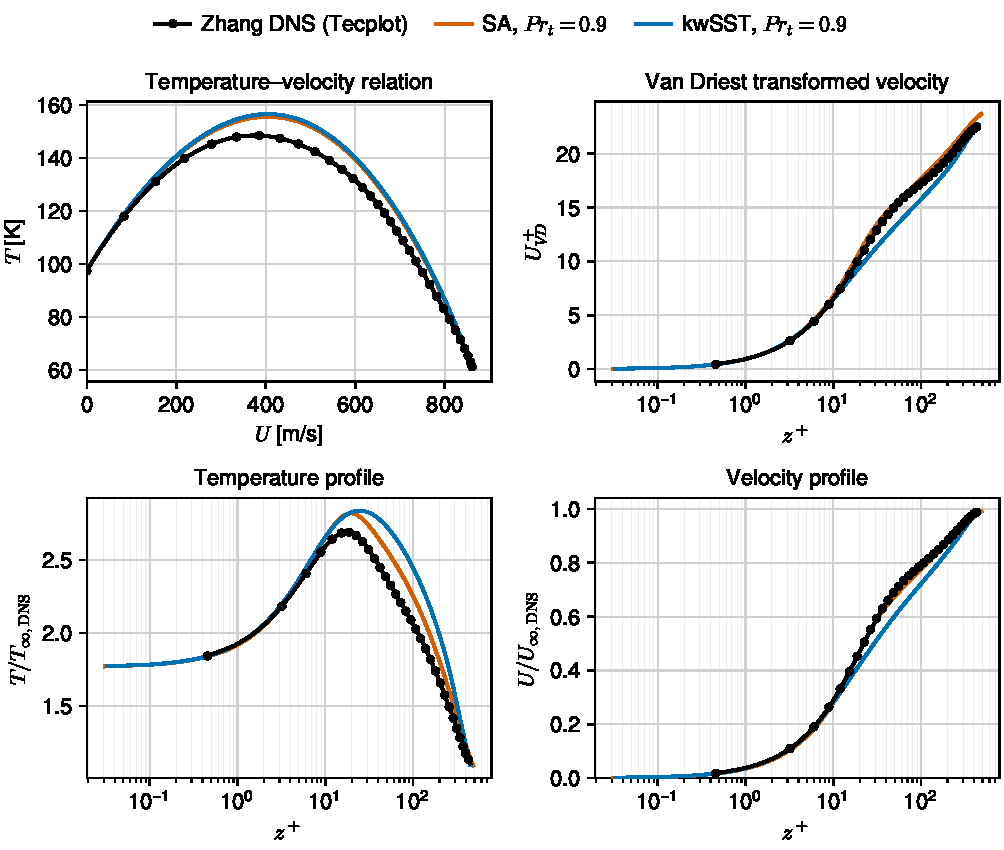
\includegraphics[width=\linewidth]{07_Error_Isolation_Results/Figures/WallResolved/M6Tw025_BL_profiles.pdf}
    \caption[M6Tw025: wall-resolved boundary layer profiles compared with DNS]{Wall-resolved Spalart--Allmaras and \(k\)--\(\omega\) SST profiles for M6Tw025 at \(Pr_t=0.9\), matched at \(Re_{\delta2}=1135\) and compared with Zhang et al.'s digital DNS profiles~\cite{zhang2018direct}. Top: dimensional temperature--velocity relation \(T(U)\) (left) and van Driest--transformed velocity \(U_{\mathrm{VD}}^+\) versus wall distance \(z^+\) (right). Bottom: normalized temperature \(T/T_{\infty,\mathrm{DNS}}\) (left) and velocity \(U/U_{\infty,\mathrm{DNS}}\) (right) versus \(z^+\). Profiles are truncated at their \(99\%\)-velocity boundary layer edge. The thermal maximum is overpredicted by both turbulence models despite differences between their velocity profiles.}
    \label{fig:wall-resolved:M6Tw025_BL_Profile}
\end{figure}

\begin{figure}[H]
    \centering
    % Figure provenance (WSL; absolute paths):
    %   Figure: /home/mgnadlinger/Duan_DNS_ZPGFP/dns_comparison_SA_kwSST/figures/Part4_LowH_M3_profiles.png
    %   Python script:
    %     /home/mgnadlinger/Duan_DNS_ZPGFP/plot_combined_dns_profiles.py
    %   Data / simulation roots (high-level):
    %     /home/mgnadlinger/Duan_DNS_ZPGFP/Martin_Duan_Part4/SA_Prt0p9/LowH_M3
    %     /home/mgnadlinger/Duan_DNS_ZPGFP/Martin_Duan_Part4/kwSST_Prt0p9/LowH_M3
    %     /home/mgnadlinger/Duan_DNS_ZPGFP/Martin_Duan_Part4/Digitizations
    %   Note: Previous thesis PNG cropped the upper two panels of the source export.
    %   Print-size replot (2026-10-19):
    %     thesis/07_Error_Isolation_Results/Figures/WallResolved/plot_wall_resolved_profiles.py
    %     Exact plotted coordinates and source hashes retained in adjacent
    %     wall_resolved_profile_data.json and wall_resolved_profile_provenance.json.
    %     Original curves/stations/panel selection preserved; 170 mm PDF, 10.5 pt text.
    % End figure provenance.
    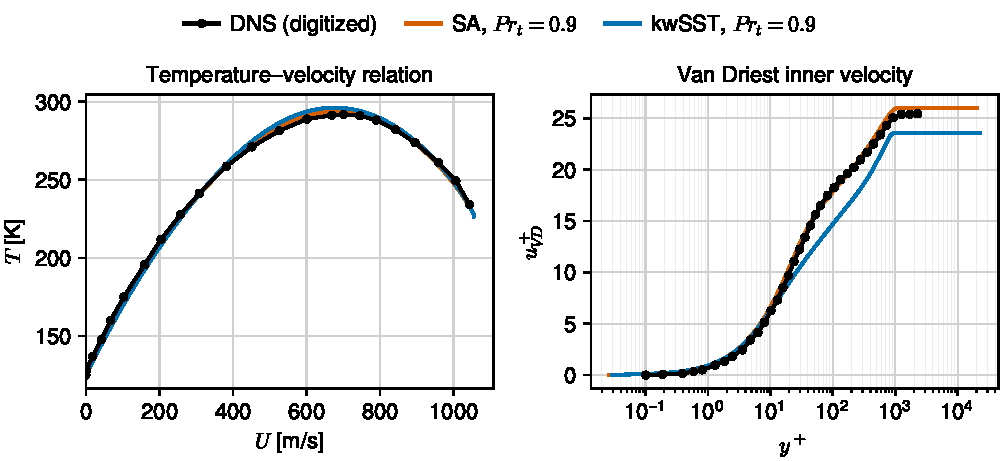
\includegraphics[width=\linewidth]{07_Error_Isolation_Results/Figures/WallResolved/Part4_LowH_M3_BL_profiles.pdf}
    \caption[LowH\_M3: wall-resolved boundary layer profiles compared with DNS]{Wall-resolved Spalart--Allmaras and \(k\)--\(\omega\) SST profiles for Martin--Duan Part~4 LowH\_M3 at \(Re_{\delta2}=1554.5\) and \(Pr_t=0.9\), compared with digitized DNS~\cite{duan2011direct_Part4}. Left: dimensional temperature--velocity relation \(T(U)\). Right: van Driest--transformed velocity \(U_{\mathrm{VD}}^+\) versus wall distance \(y^+\). The DNS wall-normal reconstruction retains the provisional boundary layer-edge endpoint assumption indicated in the plot. Both models closely reproduce the displayed \(T(U)\) relation, while their transformed velocity profiles differ.}
    \label{fig:wall-resolved:LowH_M3_BL_Profile}
\end{figure}

For M6Tw025, both Spalart--Allmaras and \(k\)--\(\omega\) SST overpredict the temperature maximum and the recovering part of the thermal profile (see Figure~\ref{fig:wall-resolved:M6Tw025_BL_Profile}). Their \(T(U)\) curves are very similar, although the transformed velocity profiles and the locations of the thermal maximum in wall units differ. SST's close wall-coefficient agreement (see Figure~\ref{fig:wall-resolved:kwSST_DNS_ZPG_FPs}) consequently coexists with a visibly incorrect thermal profile. SA, meanwhile, follows the displayed velocity profiles comparatively closely despite its thermal discrepancy. Section~\ref{subsec:erriso:rans-profile-influence} tests the consequence for wall-function heating by applying the same Li closure to the DNS and resolved SA profiles.
\par\medskip

The LowH\_M3 case presents the complementary behaviour: both models closely reproduce the displayed \(T(U)\) relation (see Figure~\ref{fig:wall-resolved:LowH_M3_BL_Profile}), yet their wall coefficients retain appreciable errors, especially for SST (see Figure~\ref{fig:wall-resolved:kwSST_DNS_ZPG_FPs} and Figure~\ref{fig:wall-resolved:SA_DNS_ZPG_FPs}). Among the selected cold-wall cases, LowH\_M3 provides the only qualitatively close agreement in the thermal \(T(U)\) relation.
\par\medskip

This distinction follows from the derivative character of the wall quantities. As described in Section~\ref{sec:openFOAM_qw_tauw}, resolved wall heat-flux and shear stress depend on the temperature and velocity gradients at the wall. A profile can agree over much of the boundary layer while retaining a different wall gradient and conversely, a similar wall gradient does not establish agreement throughout the profile. Visual comparison of \(T(U)\) therefore complements the coefficient errors and cannot replace them. The same reasoning will apply to the wall-function closures: a visually close temperature--velocity relation is insufficient to establish the accuracy of the wall quantities recovered from it.

\subsection{Evidence concerning the turbulent Prandtl number}
\label{subsec:comparative:zpg:wr-prandtl}

The similarity of the SA and SST \(T(U)\) discrepancies throughout all but one of the investigated hypersonic cold-wall ZPG FP cases motivates examination of their common thermal closure. Both extend the eddy viscosity to thermal transport through \(\kappa_t=c_p\mu_t/Pr_t\). Fixing \(Pr_t\) fixes the local ratio of modelled turbulent momentum and thermal diffusivity, even though their physical relationship may vary across a cold-wall boundary layer.
\par\medskip

Figure~\ref{fig:evaluation:turb_prandtl_comparison} compares the DNS turbulent-Prandtl-number distributions across the boundary layer with the adopted constant value of \(Pr_t = 0.9\). It is clearly visible, that much of the outer boundary layer has values of order unity - arguing for a constant \(Pr_t\) - but the near-wall regions show pronounced variation, overshoots and sign changes. This also uncovers a notable difference in the LowH\_M3 and M6Tw025 case, which may explain their difference in the ability of the turbulence model to reprduce their thermal boundary layer profile (see Figure~\ref{fig:wall-resolved:LowH_M3_BL_Profile} vs. ~\ref{fig:wall-resolved:kwSST_DNS_ZPG_FPs}). The LowH\_M3 case recovers toward values near unity after its sharp near-wall excursion, whereas the M6Tw025 distribution falls below unity over a broader part of the inner boundary layer. So while the constant \(Pr_t = 0.9\) is still a reasonable assumption for for hypersonic adiabatic wall cases and in the outer region of hypersonic cold-wall cases, it is not in the near-wall region for the majority of the hypersonic cold-wall cases. From this analysis, it is not possible to conclude that the turbulent Prandtl number is the sole cause of the observed discrepancies, but it is a plausible contributor. As discussed in later Section~\ref{subsec:comparative:zpg:case-selection} this work can also not find an immediate explanation for the difference in the turbulent Prandtl number distributions between the two cases.
\par\medskip

The sharply varying DNS values require particular care. The diagnostic \(Pr_t\) is obtained from turbulent fluxes and mean gradients, rather than being an independently measured transport constant. Duan and Martin associate its overshoots and sign changes with the crossover locations of the turbulent heat-flux and mean temperature gradient~\cite[Section~5]{duan2011direct_Part4}. Near these locations the inferred local ratio can become poorly conditioned, and a temperature maximum alone does not imply a divergence of \(Pr_t\). Such behaviour also exposes limitations of describing the turbulent thermal flux everywhere by a positive scalar diffusivity and a local temperature gradient. Directly substituting the displayed singular or negative values into the present RANS closure would therefore require a different modelling argument.

\begin{figure}[H]
    \centering
    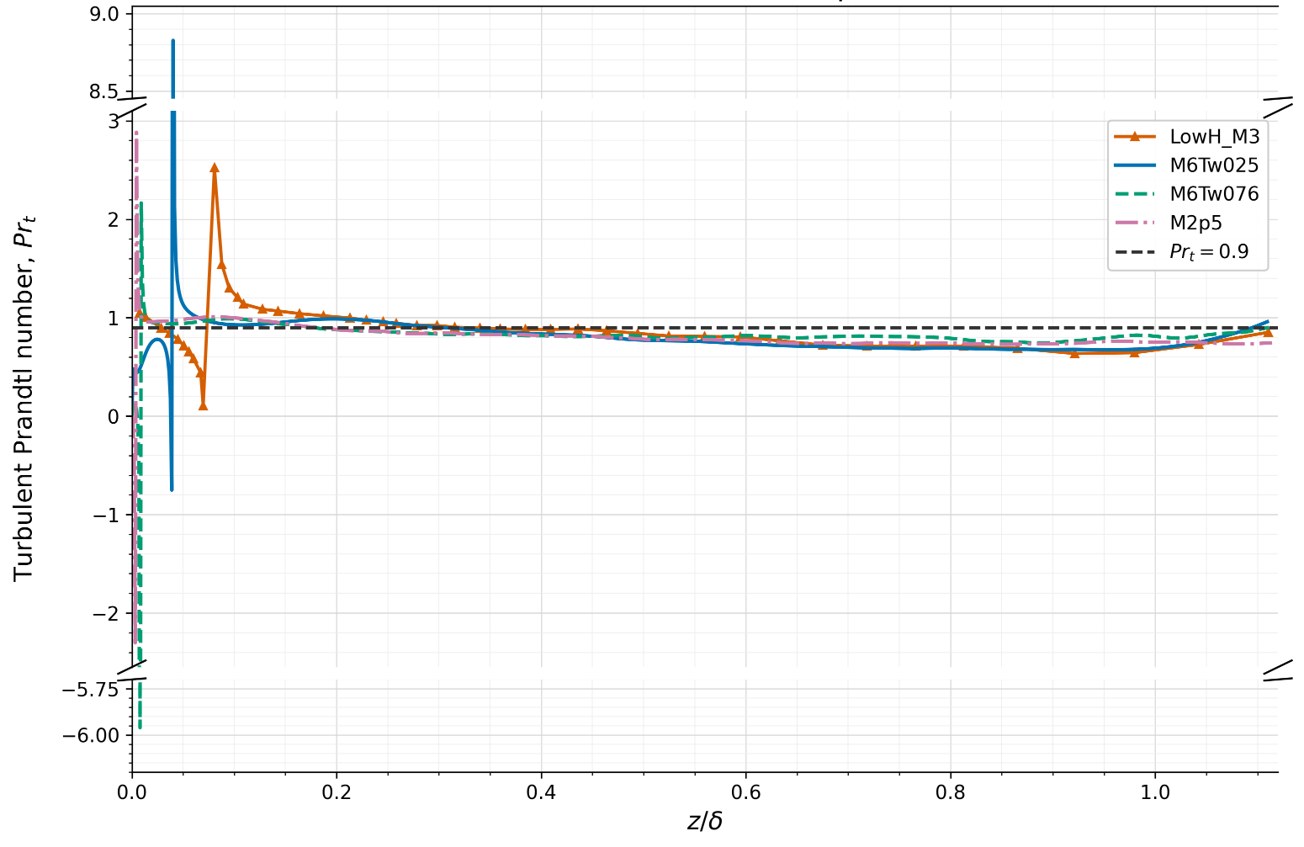
\includegraphics[width=0.8\linewidth]{06_Eval_Methodology/06_Figures/Turb_Prandtl_Number_Comparison.png}
    \caption[DNS turbulent-Prandtl-number distributions]{Turbulent Prandtl number across the whole boundary layer height, with wall-normal distance \(z\) normalized by the respective boundary layer thickness \(\delta\). M2p5, M6Tw025 and M6Tw076 use Zhang et al.'s DNS data~\cite{zhang2018direct}; LowH\_M3 uses the digitized Martin--Duan Part~4 distribution~\cite{duan2011direct_Part4}. The dashed horizontal line marks the RANS value \(Pr_t=0.9\). Breaks in the vertical axis retain the large excursions near the wall while exposing the order-unity variation over the rest of the profile. The M2p5 and M6Tw076 are adiabatic cases, whereas LowH\_M3 and M6Tw025 are strongly cold-wall cases (see Section~\ref{sec:evaluation:benchmark-cases}).}
    \label{fig:evaluation:turb_prandtl_comparison}
\end{figure}

The RANS \(Pr_t\)sensitivity calculations represented in Figure~\ref{fig:evaluation:turb_prandtl_comparison_thermal_profile} provides further evidence that the thermal closure materially affects the \(T(U)\) profile. Reducing the constant \(Pr_t\) from \(1.0\) to \(0.6\) lowers the predicted temperature maximum in both models and brings it closer to DNS. No displayed constant reproduces the entire relation: the curves retain differences on the upper,  recovering region. This aligns with the previous observation that the M6Tw025 case has a near-wall \(Pr_t\) distribution that remains below unity over a broader part of the inner boundary layer.

\begin{figure}[H]
    \centering
    % Figure provenance and typography restoration (2026-10-19):
    %   Original high-resolution export: ../Weekly 260803.pptx, slide 21,
    %     archive member ppt/media/image13.png (3189 x 1232 pixels).
    %   Retained source and reproduction script:
    %     thesis/06_Eval_Methodology/06_Figures/thermal_BL_profile_Prt_source/
    %     original_export.png, restore_typography.py and provenance.json.
    %   Original sensitivity-study data/script were not located. Curve pixels
    %     are preserved; axes/ticks/legends are replaced with larger vector text.
    %     This restores typography rather than replotting numerical data.
    % End figure provenance.
    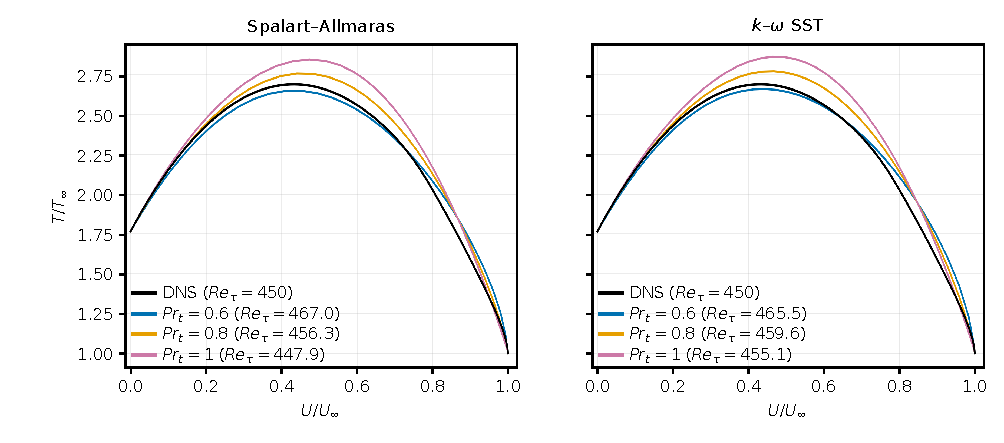
\includegraphics[width=\linewidth]{06_Eval_Methodology/06_Figures/thermal_BL_profile_Prt.pdf}
    \caption[Effect of constant \(Pr_t\) on the M6Tw025 temperature--velocity relation]{Sensitivity of the M6Tw025 mean temperature--velocity relation to constant \(Pr_t=0.6\), \(0.8\) and \(1.0\) in wall-resolved SA (left) and \(k\)--\(\omega\) SST (right). Temperature and velocity are normalized by the freestream values. The DNS reference has \(Re_\tau=450\); the RANS stations have approximately \(448\leq Re_\tau\leq467\), as listed in the legends. These stations differ from the \(Re_{\delta2}\)-matched baseline protocol. Lower \(Pr_t\) reduces the thermal maximum but does not remove the discrepancy over the complete relation.}
    \label{fig:evaluation:turb_prandtl_comparison_thermal_profile}
\end{figure}

Taken together, the DNS distributions, the similar thermal-profile errors of two different momentum closures, and the constant-\(Pr_t\) sensitivity identify the thermal closure as a plausible contributor to the discrepancies. They do not isolate it from errors in the eddy viscosity or from other modelling assumptions. Related hypersonic calculations by Huang et al. found improved temperature predictions with an algebraic turbulent-energy-flux closure compared with constant \(Pr_t\), using an algebraic momentum model~\cite{huang2020simulation}. That result supports further investigation of the thermal closure, while its different momentum model prevents direct attribution of the present SA and SST errors to \(Pr_t\) alone.
\par\medskip

\subsection{Assessment of results and comparison to existing publications}
\label{subsec:comparative:zpg:results-assessment}

Several published RANS assessments use the Zhang and Huang benchmarks included in Table~\ref{tab:evaluation:selected-cases}. They provide context for the wall-load errors and thermal-profile discrepancies found here, but common case and model names do not ensure equivalent calculations. The following comparison identifies differences in model formulation, mean-flow coupling, inflow conditions and sampling location that affect interpretation of Table~\ref{tab:wall-resolved:coefficients}.

\paragraph*{Huang et al. (2019)}

Huang et al.~\cite{huang2019assessment} assess SA and SST for M8Tw048 and report wall-coefficient errors within \(5\%\), broadly consistent with the small errors obtained here for this case. Their calculations use \(Pr_t=0.85\) and \(Re_\tau\) matching, whereas the present baseline uses \(Pr_t=0.9\) and \(Re_{\delta2}\) matching (Section~\ref{subsec:evaluation:matching-station}). Moreover, reconstructing the DNS heat-flux from the published, rounded \(-B_q\) introduces a \(\pm8.33\%\) rounding bound (Table~\ref{tab:evaluation:zhang-bq-rounding}). This limits comparisons based on that reconstruction and it is not an uncertainty estimate for Huang et al.'s underlying DNS data.

\paragraph*{Aiken et al. (2022)}

Aiken et al.~\cite{aiken2022assessment} assess SA, \(k\)--\(\omega\) BSL and SST against six Zhang and Huang benchmarks at \(Pr_t=0.9\). They report thermal-profile discrepancies similar to those in Section~\ref{subsec:comparative:zpg:wr-profiles} and identify the thermal closure as a possible contributor. Their tested freestream-turbulence variations have little downstream influence for M8Tw048. However, their SA model includes the Catris--Aupoix correction, distinct from the implementation correction in Section~\ref{subsec:ext:spalart-allmaras-of-correction}, and their original SST formulation differs from the updated version described in Section~\ref{sec:background:rans-turbulence-modelling}. They match \(Re_\tau\), while reporting similar errors with \(Re_\theta\) matching. Their Table~1 also lists total enthalpies inconsistent with the stated flow conditions, and Table~3 contains inconsistent \(Re_\theta/\theta\) values for M8Tw048. These reporting issues limit reproducibility without establishing that the imposed flow states were incorrect. Together with the formulation differences, they prevent treating agreement or disagreement as a direct code-verification result, consistent with the reporting concerns of Viti et al.~\cite{viti2007numerical}.

\paragraph*{Danis (2023)}

Danis~\cite[Figure~4.10]{danis2023direct} compares original SST skin-friction predictions with DNS for M6Tw025, M14Tw018 and M11Tw020 as functions of \(Re_\tau\), without a corresponding SST wall-heat-flux comparison. The calculations use VULCAN-CFD and cite Menter's 1994 SST model, but the turbulent Prandtl number and detailed model settings are not specified in that assessment. Differences from the present skin-friction results therefore cannot be attributed to a particular modelling or implementation choice.

\paragraph*{Vaughan et al. (2025)}

Vaughan et al.~\cite{vaughan2025paper} and Vaughan's master's thesis~\cite{vaughan2025thesis} examine overlapping Zhang and Huang cases. The thesis likewise finds cold-wall thermal-profile discrepancies at \(Pr_t=0.9\), but uses SA-neg and a vorticity-based SST limiter, rather than the present model variants. It selects sampling locations by matching the initial DNS boundary layer thickness and then advancing by the reported downstream distance, rather than matching \(Re_\tau\). This is the shifted-station approach discussed in Section~\ref{subsec:evaluation:matching-station}.
\par\medskip

For SST, Vaughan's documented mean-flow equations retain the isotropic turbulent stress, turbulent kinetic energy in total energy, and its diffusive transport, whereas the present HiSA formulation omits these contributions. Zhang et al.~\cite{zhang2021formulation} found sensitivity to these terms in shock interactions but little influence on skin-friction and velocity profiles for their single Mach-5 flat-plate. That result does not establish negligible heating sensitivity for the present cases.
\par\medskip

Vaughan also interprets the DNS freestream states as post-shock values and supplies modified pre-shock inflows~\cite[Tables~2.2--2.3]{vaughan2025thesis}. The reconstruction procedure is unspecified and a discrepancy arises for M14Tw018, where the tabulated pre-shock mean-flow total enthalpy \(c_pT+U^2/2\) exceeds the DNS value by \(4.56\%\). Table~\ref{tab:inflow-comparison} tests these inflows in the present SST implementation for four Zhang cases, retaining each run's own \(Re_{\delta2}\)-matched station. This demonstrates sensitivity to the inflow specification, but neither establishes which inflow better reproduces DNS nor reproduces Vaughan's complete setup.

% Data: /home/mgnadlinger/Zhang_DNS_ZPGFP/kwSST_Prt0p9/inflow_comparison_20261017/comparison_native_with_DNS.csv
% Extraction: add_dns_reference.py --matching native in the same directory;
% station and DNS-reference provenance: DNS_reference_native_audit.json.
\begin{table}[H]
    \centering
    \caption[Inflow sensitivity of wall-resolved SST wall loads]{Inflow sensitivity of the present wall-resolved \(k\)--\(\omega\) SST simulations against Zhang's DNS~\cite{zhang2018direct}. Original inflows use the DNS freestream conditions in Table~\ref{tab:evaluation:zhang-inflow-wall}; modified inflows use Vaughan's pre-shock values~\cite[Table~2.2]{vaughan2025thesis}. Each run is evaluated at its own \(Re_{\delta2}\)-matched station using its respective inlet density and velocity. Parentheses give \(100(\mathrm{RANS}-\mathrm{DNS})/\mathrm{DNS}\). Heat-flux is positive into the wall; shear stress is its magnitude. The M6Tw076 heat-flux reference is nominal and retained only for this sensitivity comparison, subject to the rounding and wall-temperature limitations in Section~\ref{sec:evaluation:benchmark-cases}.}
    \label{tab:inflow-comparison}
    \small
    \begin{tabular}{@{}llrr@{}}
        \toprule
        Case & Reference / inflow & \(q_w\) [\(\mathrm{kW\,m^{-2}}\)] & \(\tau_w\) [\(\mathrm{Pa}\)] \\
        \midrule
        M6Tw025 & \textbf{Zhang DNS} & \textbf{11.4888} & \textbf{28.3210} \\
        M6Tw025 & Original & 11.8290 (\(+2.96\%\)) & 29.2326 (\(+3.22\%\)) \\
        M6Tw025 & Vaughan & 11.4180 (\(-0.62\%\)) & 28.2175 (\(-0.37\%\)) \\
        \addlinespace
        M6Tw076 & \textbf{Zhang DNS} & \textbf{2.1720} & \textbf{16.2533} \\
        M6Tw076 & Original & 1.8925 (\(-12.87\%\)) & 15.3712 (\(-5.43\%\)) \\
        M6Tw076 & Vaughan & 1.8585 (\(-14.43\%\)) & 15.1801 (\(-6.60\%\)) \\
        \addlinespace
        M8Tw048 & \textbf{Zhang DNS} & \textbf{4.5495} & \textbf{13.2915} \\
        M8Tw048 & Original & 4.6231 (\(+1.62\%\)) & 13.3289 (\(+0.28\%\)) \\
        M8Tw048 & Vaughan & 4.5881 (\(+0.85\%\)) & 13.2067 (\(-0.64\%\)) \\
        \addlinespace
        M14Tw018 & \textbf{Zhang DNS} & \textbf{10.3028} & \textbf{12.1640} \\
        M14Tw018 & Original & 11.7582 (\(+14.13\%\)) & 14.0633 (\(+15.61\%\)) \\
        M14Tw018 & Vaughan\textsuperscript{*} & 12.3612 (\(+19.98\%\)) & 14.3311 (\(+17.82\%\)) \\
        \bottomrule
    \end{tabular}
    \par\smallskip
    \begin{minipage}{\linewidth}
        \footnotesize
        \textsuperscript{*} Vaughan's tabulated M14Tw018 pre-shock mean-flow total enthalpy \(c_pT+U^2/2\) is \(4.56\%\) higher than that of the DNS freestream state.
    \end{minipage}
\end{table}

\paragraph*{Cheng et al. (2026)}

Cheng et al.~\cite{cheng2026reynolds} use OpenFOAM-v2312 and the HiSA solver framework to investigate energy closures with the Durbin--Yin \(k\)--\(\omega_0\) model, including additional SST--\(\omega_0\) tests. Their baseline therefore differs from the present SST model even before the proposed energy-closure corrections. Their stated energy equation includes turbulent-kinetic-energy transport~\cite[Eq.~2.7]{cheng2026reynolds}, which is absent from the present HiSA formulation. The paper does not specifically state having performed the corresponding solver modifications outside of the stated RANS equations. Shared solver ancestry consequently does not establish equivalent mean-flow coupling. Station selection adds another difference, although the present tests in Tables~\ref{tab:evaluation:matching-station-bq} and~\ref{tab:evaluation:matching-station-ch} give changes below \(1\%\) in \(-B_q\) and \(2\%\) in \(C_h\) between the shifted and \(Re_{\delta2}\)-matched stations. Their Table~5 also normalizes \(B_q\) with DNS wall quantities, whereas Table~\ref{tab:wall-resolved:coefficients} uses each solution's own wall state. These values require consistent normalization before comparison.

\paragraph*{Implications for the present assessment}

The literature supports treating the present discrepancies as part of a broader difficulty in predicting cold-wall boundary layers with conventional RANS closures. It does not provide an equivalent setup for direct code verification or isolate the cause of differences in wall loads. In particular, the thermal-profile deficiencies reported by Aiken and Vaughan reinforce the evidence in Sections~\ref{subsec:comparative:zpg:wr-profiles} and~\ref{subsec:comparative:zpg:wr-prandtl}, without establishing constant \(Pr_t\) as their sole cause. The subsequent wall-function assessment therefore retains both DNS and the present wall-resolved SA solution as distinct references, as defined in Table~\ref{tab:erriso:reference-hierarchy}.

\subsection{Selection of cases for detailed wall-function assessment}
\label{subsec:comparative:zpg:case-selection}

M6Tw025 and LowH\_M3 are retained for the detailed coupled wall-function analysis because they expose different relationships between wall-coefficient and profile accuracy. M6Tw025 supplies digital DNS profiles for a strongly cooled Mach-6 boundary layer and exhibits a clear thermal-profile discrepancy in both RANS models. It therefore tests the wall functions when their analytical thermal relation is coupled to a resolved RANS field that already differs from DNS. Its detailed reference profiles also permit an independent prescribed-profile closure assessment, subject to the heat-flux reporting limitations stated above.
\par\medskip

LowH\_M3 supplies a cold-wall supersonic comparison in which the resolved RANS \(T(U)\) relation closely follows the digitized DNS. This reduces the pronounced thermal-profile mismatch present in M6Tw025 and makes the case useful for examining additional errors introduced by the wall function and the CFD mesh. The nonzero wall-coefficient errors remain part of its baseline. In the subsequent prescribed-profile calculations, the resolved SA field is used as the LowH\_M3 input, so those closure errors measure consistency with SA rather than an independent reconstruction of DNS wall quantities.
\par\medskip

The contrasting thermal-profile accuracy of LowH\_M3 and M6Tw025 cannot be attributed to the models' incompressible origins alone. The corresponding DNS studies~\cite{zhang2018direct,duan2011direct_Part4} report approximate Morkovin-type similarity and outer-layer agreement with modified strong Reynolds analogies for both cases (ref. Section \ref{subsec:background:SRA-Morkovin}). This weakens an explanation based on a fundamental loss of applicability between the two flow conditions, without excluding differences in intrinsic compressibility, mean-property gradients or thermal transport. The cause of the contrast remains unresolved, with the following analysis therefore examining the shared constant turbulent Prandtl number as a possible contributor.
